%
% Apunte de Sistemas Operativos
% Copyright (C) 2014 Esteban De La Fuente Rubio (esteban[at]delaf.cl)
%
% Permission is granted to copy, distribute and/or modify this document
% under the terms of the GNU Free Documentation License, Version 1.3
% or any later version published by the Free Software Foundation;
% with no Invariant Sections, no Front-Cover Texts, and no Back-Cover Texts.
% A copy of the license is included in the section entitled "GNU
% Free Documentation License".
%
% Link: http://www.gnu.org/copyleft/fdl.html
%

% CAPÍTULO HISTORIA
\chapter{Historia}
\label{historia}
Los sistemas operativos han evolucionado enormemente desde sus inicios, durante
este capítulo se mencionarán aspectos relacionados con los diferentes tipos de
sistemas operativos existentes o que han existido junto a lo que se ha logrado a
lo largo de los años.

\section{Tipos de sistemas}

\subsection{Érase una vez (50's)}
Cuando se comenzaron a utilizar grandes máquinas para realizar cómputos no
existía un sistema operativo propiamente tal, solo había hardware y las
aplicaciones (trabajos o \textit{jobs}) de los usuarios. Se leía el programa a
ejecutar y se ejecutaban sus instrucciones de manera secuencial.

Las aplicaciones en esta época debían incluir todo el código, incluyendo aquel
para manejar cada uno de los dispositivos de hardware que la máquina tenía
disponible. Se debe acceder directamente al espacio de direcciones, tanto de
memoria principal como memoria secundaria. No existe estructura de directorios
ni archivos en la memoria.

Si se desea ejecutar una nueva aplicación, se debe cargar el nuevo trabajo y la
máquina debe ser reiniciada. La depuración de la aplicación se realiza de forma
presencial, observando las salidas indicadas mediante las luces del computador.
El equipo es utilizado solo por un usuario al mismo tiempo y por un período
largo de tiempo para realizar todas las tareas involucradas.

El principal problema de esta etapa es el bajo uso del hardware disponible,
donde existe mucho tiempo que no es utilizado en cómputo. Siendo que el
componente caro es el hardware y no el programador, se debe buscar una solución
a este problema.

A pesar de lo anterior, y lo rudimentario que podría parecer frente a los
computadores que actualmente existen, estas máquinas eran capaces de procesar
cálculos mucho más rápido que un gran número de calculistas trabajando en
conjunto.

\subsection{Sistemas por lotes (fines 50's)}
En un sistema operativo por lotes se requiere que todos los componentes del
programa, ya sea el mismo código del programa, los datos y las llamadas al
sistema que permiten usar el hardware sean introducidos, comúnmente, mediante
tarjetas perforadas, ver figura \ref{fig:lotes}, de 80 caracteres cada una. Este
conjunto de instrucciones es conocido como un trabajo o un \textit{job}, el cual
poseía poca o ninguna interacción con el usuario.

\begin{figure}[htbp]
\centering
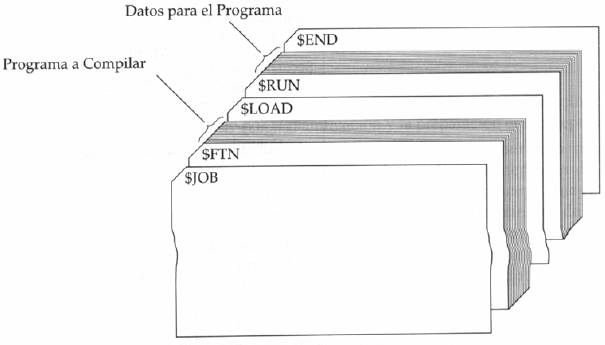
\includegraphics[scale=.7]{img/C02_historia/lotes.png}
\caption{Tarjetas de un sistema por lotes}
\label{fig:lotes}
\end{figure}

Este tipo de sistemas operativos era útil con programas que fuesen largos y sin
interacción con el usuario. Donde un operador recibía los trabajos de los
programadores y los introducía en la máquina, estos eran procesados en orden
FIFO (First In First Out), o sea el primer trabajo que llegaba era el primero
que se procesaba.

La planificación del procesador y administración de la memoria es simple, en el
primer caso bastaba pasar el control del mismo al \textit{job} y que este lo
devolviera al terminar su ejecución. En el caso de la memoria también la
administración era simple, ya que el espacio se dividía en dos partes, una para
el monitor residente (el sistema operativo) y otra para el trabajo en
ejecución.

Al aparecer el monitor residente, también aparece el concepto de API, donde el
programador ya no debía escribir todas las instrucciones para acceder al
hardware, sino que se le entregaba ya una herramienta para facilitar su
trabajo.

Si ocurría algún error durante la ejecución del trabajo se entregaba al
programador un \textit{dump} de la memoria, de tal forma que este pudiera
corregir el error en el programa y volver a entregar un conjunto de tarjetas
corregidas para su ejecución. Esto evitaba que el programador tuviese que estar
frente al computador para depurar su código.

A pesar de que el computador se encontraba más tiempo ocupado, porque siempre
que hubiesen tarjetas se estarían procesando, su componente más costosa, la CPU,
que es más rápida comparada con los dispositivos de entrada o salida de datos,
no se encontraba necesariamente ocupada todo el tiempo. Las tareas de lectura y
escritura son bloqueantes y mantienen a la CPU en un ciclo de
\textit{busy-waiting}. Lo anterior significa que mientras se está leyendo o
escribiendo, la CPU no puede realizar otras tareas (ya que espera que la lectura
o escritura termine).

\subsection{Sistemas de operación \textit{offline} (60's)}
La idea principal tras las operaciones fuera de línea, o \textit{offline},
corresponde a la lectura y escritura de los elementos utilizados en los sistemas
operativos por lotes, o sea las tarjetas, de forma externa al computador
principal. Lo anterior buscaba no utilizar el procesador más caro disponible en
tareas lentas (como leer tarjetas), sino utilizar otras unidades que traspasaban
las tarjetas perforadas a cintas y luego estas cintas eran cargadas en la
máquina principal.

Análogamente a lo explicado, la salida del computador principal era generada en
cintas magnéticas, las cuales en una etapa posterior a la ejecución del programa
eran llevadas a un equipo de impresión donde se obtenía una salida que se
entregaba al programador.

Con este sistema fuera de línea, se lograba un mejor rendimiento del procesador
principal, utilizándolo para tareas de cómputo y dejando las tareas de lectura y
escritura a otros equipos más económicos.

La cantidad de máquinas periféricas utilizadas dependerá de la capacidad del
procesador, o sea, mientras existiera tiempo de CPU sin uso, se podían seguir
agregando cintas al computador principal. Una vez el tiempo de CPU ya había
alcanzado su uso constante, no tenía sentido agregar más impresoras (o lectoras)
ya que no se generarían más cintas para imprimir por unidad de tiempo.

El trabajo solo entrega el control del sistema al monitor residente en caso de
término, que se requiera algún servicio de entrada o salida o en caso de error.

A pesar de esta mejora en la velocidad de lectura y escritura, el procesador,
mientras se realizan dichas operaciones, continúa estando ocioso, sigue
existiendo problema de \textit{busy-waiting} en cintas. Consideremos que para
leer una línea de la cinta se tomaban 80 caracteres (misma cantidad que una
tarjeta perforada) y se escribían de a 80 caracteres (en caso de cintas) y de a
132 caracteres en impresoras. El leer una línea implicaba hacer girar la cinta,
lo cual generaba inercia en la cinta y hacía que hubiese que ajustarla
(retrocediendo) para leer la próxima línea en el futuro.

Adicionalmente existía un mayor tiempo para los programadores, que debían
esperar que sus programas fueran traspasados a cinta, ejecutados, luego los
resultados traspasados a cinta e impresos.

\subsection{Sistemas con \textit{buffering} (60's)}
Para ayudar a solucionar el problema de leer línea a línea las instrucciones de
una cinta se empezaron a leer de a 10 líneas, o sea de a 800 caracteres, lo cual
permitía disminuir los tiempos de lectura. En vez de leer de a una línea, se
leían 10 considerando que en algún momento futuro esas líneas podrían ser
utilizadas, las líneas leídas eran guardadas en un \textit{buffer} a la espera
de ser solicitadas. Por lo tanto cuando eventualmente el trabajo requería una
línea, esta era leída desde el \textit{buffer} y no desde la cinta, reduciendo
los tiempos.

De la misma forma para escribir en la cinta, se guardaba en un \textit{buffer}
lo que se quisiera escribir, una vez lleno este \textit{buffer} se escribía todo
en la cinta de una vez.

Mediante el uso de canales, uno para la lectura y otro para la escritura, se
podían conseguir mejoras en los tiempos y rendimiento de la CPU. Ya que la tarea
de leer y llevar al \textit{buffer} o sacar del \textit{buffer} y escribir la
realizaban los canales propiamente tal, y la CPU no era necesaria durante toda
la operación de E/S, con lo que la misma podía ser utilizada para tareas de
cómputo.

El rendimiento de esta técnica dependerá básicamente de si el proceso es
intensivo en CPU, en E/S o es igual en ambos casos. A pesar de lo anterior el
porcentaje de utilización de CPU, gracias al \textit{buffering} y uso de canales
aumentará.

El principal problema de esta técnica sigue siendo el tiempo de espera extra
agregado al tener que leer las tarjetas y cargarlas en cintas y luego las cintas
imprimirlas, esto básicamente por el transporte de un sistema periférico al
computador principal.

\subsection{Sistemas de operación \textit{online} (60's)}
En este tipo de sistemas la lectura de tarjetas e impresión de resultados ya no
es realizada en equipos periféricos. Las lectoras e impresoras se conectan
directamente al computador central y hacen uso de los canales de E/S que se
agregaron en el sistema con \textit{buffering}. Esto fue posible gracias a la
aparición de discos duros los cuales contenían la entrada de los trabajos y
almacenaban las salidas de los mismos.

En este tipo de sistemas el monitor residente es quien se encarga de leer
tarjetas y dejarlas en el disco y de imprimir los resultados. Para ejecutar un
trabajo debe haber sido leído completamente al disco, así mismo para imprimir
los resultados de un trabajo este debe haber terminado su ejecución habiendo
dejado la salida en el disco.

Esto mejora el tiempo de proceso de un trabajo, ya que no se deben utilizar
lectores o impresoras externas al computador principal, ahorrando tiempo en el
traspaso físico de las mismas de un equipo a otro.

El problema sigue siendo la ociosidad del procesador cuando se deben realizar
operaciones de entrada o salida.

\subsection{Sistemas multiprogramados (fines 60's)}
El principal problema con un sistema de operación \textit{online} es que la CPU
no está siendo utilizada todo el tiempo, esto a pesar que pueden existir
trabajos que pudiesen ser atendidos. Esto es básicamente porque no se permite la
ejecución de más de un trabajo en ``paralelo'' y se debe esperar a que uno
termine para iniciar otro.

En este tipo de sistemas se aprovecha el tiempo de E/S para ejecutar otros
trabajos. Durante esta época aparece el concepto de planificación de
procesos/trabajos (o \textit{scheduling}) y con esto el concepto de Sistema
Operativo. Ya que varios procesos deben ejecutarse, todos ellos deben estar
residentes en memoria principal. La multiprogramación implica multiprocesos, o
sea programas se ejecutan de forma ``paralela'', ver figura
\ref{fig:multiprogramado}.

\begin{figure}[htbp]
\centering
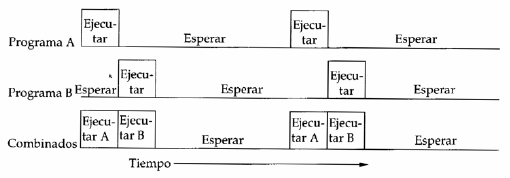
\includegraphics[scale=1.]{img/C02_historia/multiprogramacion.png}
\caption{Sistemas por lotes vs sistema multiprogramado}
\label{fig:multiprogramado}
\end{figure}

El principal problema es la no existencia de un entorno protegido para la
ejecución de los procesos, si un proceso cometía algún error podía hacer que
todo el sistema fallase.

\subsection{Máquinas o procesadores virtuales}
En este tipo de máquinas, se da soporte para la emulación de varias máquinas o
procesadores a partir de un solo procesador real. Cada máquina virtual entrega
al proceso un entorno protegido, frente a otras máquinas virtuales, de tal forma
que lo ejecutado en dicho entorno solo afecta a esa máquina virtual.

El tiempo de CPU utilizado por cada máquina es una tajada de tiempo del
procesador real. Con esto se logra el mayor rendimiento del computador,
utilizando multiprogramación, ya que la CPU siempre estará atendiendo a alguien
que lo requiera.

El problema aquí comienza a ser la baja productividad de los programadores. Lo
tiempos de ejecución total de un proceso sigue siendo alto, y la depuración de
los trabajos comienza a tomar importancia como problema.

\subsection{Sistemas de tiempo compartido (70's)}
Los sistemas de tiempo compartido corresponden a entornos multiprogramados y
multiusuario, los cuales entregaban un mejor tiempo de respuesta. Los usuarios
(programadores) pueden trabajar de forma interactiva con los computadores
mediante terminales conectadas a ellos. O sea, vuelven a trabajar directamente
con el computador, como lo hacían en los inicios, el operador ya no existe.

Cada programador dispone de una terminal con una consola, donde puede realizar
una depuración de forma más rápida, no debiendo esperar la entrega de los
resultados de la ejecución de su programa impresos.

En un sistema de tiempo compartido los usuarios comparten recursos, por lo cual
se debe hacer un reparto equitativo de los mismos y además contar con sistemas
de protección para ellos. Ahora se habla de sesiones de usuarios y no de
trabajos.

El problema aquí surge con la cantidad de usuarios y procesos que estos
ejecutan, donde el procesador no es capaz de atender a infinitos usuarios y el
sistema puede ir degradándose con cada nuevo que entra. Esto ya que el recurso
CPU que realiza los cómputos y el recurso memoria que se requiere para mantener
los procesos en ejecución son limitados.

\subsection{Computadores personales}
Gracias al uso de componentes cada vez más pequeños se logró empezar a
comercializar microprocesadores, los cuales permitían, por su bajo costo, que
fuesen adquiridos por usuarios personales. De esta forma ya no se requería
compartir el recurso CPU o memoria con múltiples usuarios, sino que cada usuario
(o programador) disponía de un equipo dedicado a sus labores.

Originalmente los computadores personales, destinados al uso por parte de un
único usuario, no requerían características de sistemas de tiempo compartido.
Con esto su diseño era más simple y requerían menos soporte del hardware para su
funcionamiento. Un ejemplo de este tipo de sistema operativo es MS-DOS.

Cada usuario posee su propia máquina, sin embargo el compartir datos entre
máquinas resultaba un proceso complicado. Cada máquina debía tener su propia
impresora y/o lectora de discos.

\subsection{Redes de computadores personales (80's)}
A mediados de los 80's surgen las redes de computadores personales, bajo esta
modalidad los usuarios podían compartir discos e impresoras con otros equipos y
de esta forma economizar en la compra de recursos.

Este esquema utiliza uno de los equipos como servidor de disco y/o impresora, y
los demás computadores se conectan vía red a este. Los usuarios conectados a
estas terminales, veían el disco o la impresora como si estuviese conectada en
su equipo.

Ya que el sistema operativo utilizado, en realidad un monitor residente, no
poseía características de protección es que era poco recomendable ejecutar
aplicaciones de usuario en el servidor, ya que la caída de la aplicación podría
hacer que todo el sistema fallase.

Las primeras redes solo permitían compartir directorios en modo solo lectura.

\subsection{Sistemas en tiempo real}
Este tipo de sistemas corresponde a los utilizados en aplicaciones de tiempo
real, donde los tiempos de respuesta a eventos del mundo físico son críticos.
Por ejemplo el uso en control de tráfico o procesos industriales.

Deben poseer tiempo de respuestas muy rápidos, para esto es requisito que los
procesos residan permanentemente en memoria principal. Adicionalmente cualquier
interrupción debe ser atendida inmediatamente. No se garantiza que se reciba de
forma inmediata, pero si en un tiempo muy acotado.

Existen variantes de GNU/Linux que están orientadas a sistemas operativos en
tiempo real.

\subsection{Sistemas distribuídos}
Corresponden a un conjunto de estaciones de trabajo o \textit{terminales
inteligentes} conectadas entre sí para trabajar de manera conjunta y como una
sola. Este modo de operación ha sido influenciado por el decaimiento del costo
de los procesadores, donde es más barato tener dos CPU funcionando conjuntamente
que una sola CPU del doble de velocidad.

Se hace uso de las redes de computadores, donde cada nodo de la red es una pieza
del computador conformado. Con esto se consigue una serie de ventajas tales como
alto rendimiento, alta disponibilidad, balanceo de carga y escalabilidad.

\subsection{Sistemas multiprocesadores}
Un sistema con múltiples procesadores permite la ejecución real en paralelo de
al menos dos procesos, considerando que como mínimo existirán dos procesadores.
En estricto rigor, y por definición de Intel, son \textit{cores} o (núcleos),
donde un procesador puede tener uno o más \textit{cores}. Quedando el concepto
de procesador o CPU como el chip y \textit{core} como el componente de la CPU
que ejecuta los procesos.

Cuando el número de procesos en ejecución supera el número de \textit{cores} se
debe recurrir al uso de algún mecanismo de planificación de procesos, donde se
deberá, al igual que en sistema monoprocesador, compartir el tiempo de CPU entre
los interesados.

Se hablará de tiempo de CPU durante el texto, pero recordar que nos estaremos
refiriendo a los \textit{cores} que están en la CPU.

\section{Tendencias últimas dos décadas}

Durante las últimas dos décadas, o sea desde los 90's, han existido diversas
tendencias en lo referente al desarrollo de sistemas operativos.

El gran crecimiento que han experimentado las redes computacionales junto a las
velocidades de acceso a Internet han permitido un mayor uso de computación
distribuida, mediante el uso de plataformas multiprocesadoras y procesadores
conectados en red.

El área de sistemas multimedia, datos más sonido más imágenes ha experimentado
un alto desarrollo. Se están desarrollando cada vez dispositivos de entrada más
rápidos y eficientes como los sistemas de reconocimiento automático de voz o
imágenes. Dichos sistemas tienen directa relación con los mencionados como
sistemas de tiempo real.

Adicionalmente la tendencia va hacia el diseño e implementación de sistemas
abiertos, tales como:

\begin{itemize}

	\item Normas de comunicación abiertas, como el modelo de referencia OSI.

	\item Normas de Sistemas Operativos abiertos como GNU/Linux.

	\item Normas de interfaces de usuario abiertas, como el sistema de
	ventanas X desarrollado por MIT.

	\item Normas de aplicaciones de usuario abiertas, como las entregadas
	por la FSF\footnote{Free Software Foundation /
	\url{http://www.gnu.org/licenses/gpl.html}}.

\end{itemize}

\section{Logros}
Durante los años de desarrollo se han obtenido diferentes logros, que perduran
en los sistemas hasta hoy en día. A continuación se mencionan brevemente estos,
en capítulos posteriores se discutirá en detalle cada uno de ellos.

\subsection{Procesos y memoria}
Un proceso corresponde, en principio, a cualquier programa en ejecución. Este
posee diversos estados, donde lo más común es encontrar: ejecución (proceso en
cpu), bloqueado (en espera de un recurso) y listo (esperando entrar a cpu).

Cualquier proceso requerirá si o si al menos el uso de memoria principal y CPU,
adicionalmente puede requerir utilizar otros dispositivos, en general cualquiera
destinado a operaciones de entrada y salida. Esto implicará que diversos
procesos podrán tratar de acceder a un mismo recurso al mismo tiempo, por lo
cual existirá competencia por dicho recurso. Para esto, a lo largo de los años,
se han diseñado diversos algoritmos que permiten al sistema operativo decidir
que proceso utilizará que recurso.

Además un proceso para funcionar requerirá algo más que su código, un proceso
estará formado por el programa o código, sus datos y un contexto (o descriptor
del proceso).

Finalmente el sistema operativo debe ser capaz de prevenir o mitigar los
problemas más comunes correspondientes a \textit{data races}, \textit{deadlock}
y \textit{starvation}. Para esto, existen mecanismos de sincronización que se
pueden utilizar.

\subsection{Seguridad y protección}
Se debe garantizar la protección de los procesos en ejecución, se mencionó ya
que sistemas operativos de tiempo compartido debían proteger a los procesos
corriendo, ya que múltiples usuarios podrían estar trabajando en la máquina.
Específicamente se deben implementar políticas que permitan controlar el acceso
a un recurso solicitado por más de un proceso, a este recurso se le conocerá
como \textbf{sección crítica} y algunas medidas que se pueden tomar son:

\begin{itemize}

	\item No compartición: procesos se encuentran aislados.

	\item Compartición solo como lectura, para escribir un recurso se
	requieren mecanismos (o condiciones) especiales.

	\item Subsistemas confinados: similar a una protección por ocultación
	donde un proceso evita que otros sepan como opera.

	\item Diseminación controlada: en este caso existen credenciales de
	seguridad para acceder a los recursos, por lo cual se especifica quien
	podrá y quien no podrá acceder al recurso.

\end{itemize}

\subsection{Gestión de recursos}
La gestión de recursos corresponde a como se deberán asignar los recursos a un
proceso que los solicite, considerando para esto que deberá existir algún tipo
de planificación que determine el orden en que serán atendidas las solicitudes.
Se deben considerar los factores:

\begin{itemize}

	\item Equidad: igualdad de preferencias frente a una solicitud.

	\item Sensibilidad: poder priorizar ciertos procesos.

	\item Eficiencia: maximizar la productividad y minimizar los tiempos de
	respuestas.

\end{itemize}

Más adelante se hablará de la planificación de CPU y como el sistema operativo
asigna este recurso a un proceso, se deberá considerar que conceptos mencionados
para la CPU son análogos a los utilizados en la planificación de otro tipo de
recursos.

\subsection{Estructura del sistema}
La estructura o arquitectura del sistema, determinará como se comportará y que
capacidades podrá el sistema operativo entregar a los procesos y usuarios que
están ejecutándose sobre el.

Es importante mencionar que la estructura del software utilizada dentro del
sistema operativo puede afectar considerablemente el funcionamiento de este. No
será lo mismo una rutina programada de cierta forma que de otra, una puede ser
más o menos eficiente dependiendo de la implementación realizada. Así mismo un
sistema con más o menos instrucciones no significa que sea un sistema más o
menos eficiente, ni mucho menos más o menos simple. Ya se habrá visto en
lenguajes de programación que existen instrucciones que utilizan muy pocas
líneas, sin embargo son difícilmente entendibles.

Se deberá dividir el sistema operativo, de tal forma que cada una de las partes
de este cumpla una función específica. Si bien se puede tener un único sistema
que implemente todas las funcionalidades (este es el caso de un sistema
operativo monolítico), aun así internamente deberá estar organizado de tal forma
que sea sencillo de mantener y programar. De no realizarse lo anterior de forma
correcta podrían existir problemas con los tiempos de entrega del software,
fallos y rendimiento en el momento de poner en funcionamiento un nuevo sistema.

El capítulo \ref{estructura} discute los conceptos de la estructura del sistema
operativo en un nivel más profundo.

\section{Ejercicios y preguntas}
\begin{enumerate}

	\item ¿Cuándo es recomendable el sistema operativo por lotes?.

	\item Describa las ventajas de un sistema de operación \textit{offline}
	versus un sistema operativo por lotes.

	\item ¿Cuál es el problema de los sistemas de operación \textit{offline}
	que se soluciona en uno con \textit{buffering}?

	\item Indique la característica que hace a un sistema multiprogramado
	ser más eficiente que sus predecesores.

	\item En un sistema de tiempo compartido ¿cuántos usuarios pueden correr
	sus programas al mismo tiempo?.

	\item ¿Cuál es la principal característica de un sistema operativo en
	tiempo real?.

	\item ¿Quién inicio el proyecto GNU?.

	\item ¿Quién inicio el proyecto Linux?.

	\item ¿Cuáles son las 4 libertades que entrega el software libre?.

	\item ¿Qué es un proceso?.

	\item Un proceso ¿es solo código?.

	\item ¿Qué se conoce como sección crítica?.

	\item Explique los conceptos de equidad, sensibilidad y eficiencia.

\end{enumerate}

\section{Referencias}
\begin{itemize}

	\item Sistemas Operativos, Segunda Edición, Andrew Tanenbaum, Capítulo
	1.2.

	\item Sistemas Operativos, Quinta Edición, Abraham Silberschatz y Peter
	Baer Galvin, Capítulo 1.

	\item Sistemas Operativos, Segunda Edición, William Stallings, Capítulo
	2.

\end{itemize}
